\subsection{IASI Band 1 (645-1210\invcm)}
%----------------------------------------

\subsubsection{WVO-derived profiles}
%...................................
The difference between the WVO transmittance sets is whether the effective water vapour or ozone transmittances are used. The residuals indicate that the effective water vapour transmittances suffer less from negative optical depths. Inspection of the indivudal transmittance profiles shows this to be the case. An example for profile 1 and frequency 1062.75\invcm{} is shown in figure \ref{fig:iasiB1.wvo_tauprofile_p1_f1062.75}. An additional consideration is the magnitude of the absorption of other components. For the example shown in figure \ref{fig:iasiB1.wvo_tauprofile_p1_f1062.75}, the water vapour absorption is quite large (centred on a water vapour line in the ozone band), but is not large enough (and does not occur high enough in the atmosphere) to saturate and thus negate any ill-effects of the correct effective ozone transmittance profile.
\begin{figure}[htp]
  \centering
  \includegraphics[scale=0.8]{graphics/iasiB1/iasiB1.wvo_tauprofile_p1_f1062.75.eps}
  \caption{IASI band 1 WVO-derived transmittance profiles for UMBC dependent set 1, $f$=1062.75\invcm{}. Panel (e) shows the ``turnaround'' in the effective ozone transmittance profile (and its ``correction'') that is used in the WVO1 set. The LBL-derived ozone transmittance profile is used in the WVO2 set.}
  \label{fig:iasiB1.wvo_tauprofile_p1_f1062.75}
\end{figure}


\subsubsection{DOZ-derived profiles}
%...................................
An example of the transmittance profiles for profile 1 and frequency 730.25\invcm{} are shown in figure \ref{fig:iasiB1.doz_tauprofile_p1_f730.25}, where the effective ozone transmittance (used in the WVO1 set) in panel (e) again shows the ``turnaround'' effect at about 200hPa. The LBL-derived ozone transmittance (used in the WVO2 set) does not exhibit the same behaviour.
\begin{figure}[htp]
  \centering
  \includegraphics[scale=0.8]{graphics/iasiB1/iasiB1.doz_tauprofile_p1_f730.25.eps}
  \caption{IASI band 1 DOZ-derived transmittance profiles for UMBC dependent set 1, $f$=730.25\invcm{}. Panel (e) shows the ``turnaround'' in the effective ozone transmittance profile (and its ``correction'') that is used in the DOZ1 set. The LBL-derived ozone transmittance profile is used in the DOZ2 set.}
  \label{fig:iasiB1.doz_tauprofile_p1_f730.25}
\end{figure}


\subsubsection{WVD-derived profiles}
%...................................
